\section{Situazioni Problematiche}

\begin{frame}{Punti Critici}
  Sono state incontrate diverse criticità:

  alcune dovute alle limitazioni della piattaforma

  altre, invece, più concettuali
\end{frame}
\begin{frame}{Cricità dovute alla piattaforma}
  \begin{itemize}[<+- | alert@+>]
    \item{Gestione del ciclo delle fasi}
          \begin{itemize}
            \item Decidim non consente di "resettare" i processi
            \item Moduli non disponibili nell'installazione di lavoro
          \end{itemize}
  \end{itemize}
\end{frame}
\begin{frame}{}
  \begin{wrapfigure}{r}{0.50\textwidth}
    \centering
    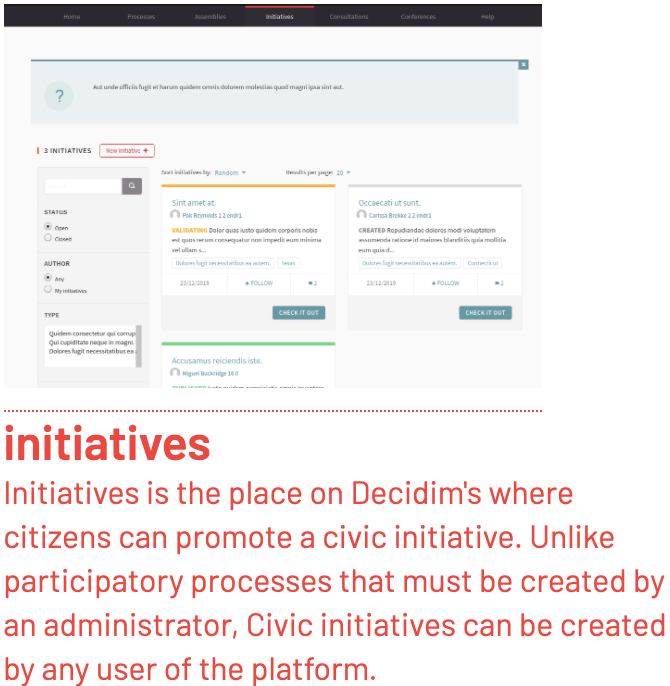
\includegraphics[width=0.50\textwidth]{iniziative}
  \end{wrapfigure}
  Il modulo iniziative avrebbe potuto fornire ai cittadini la possibilità di eleggere un responsabile in contesti autogestiti
\end{frame}
\begin{frame}{Cricità "concettuali"}
  \begin{itemize}[<+- | alert@+>]
    \item Organizzazione e aggiornamento sullo stato dei lavori di proposte autogestite
          \begin{itemize}
            \item Risolvibile con l'elezione di un responsabile
            \item Meglio se gestita in una zona apposita organizzata in stile \emph{Github}
          \end{itemize}


    \item Gestione dell'autenticazione
  \end{itemize}

\end{frame}
\begin{frame}{Gestione dell'autenticazione - Un'idea}
  \emph{Decidim} supporta la gestione dei permessi per i singoli componenti/fasi

  Una di queste prende il nome di \emph{Verifica delle autorizzazioni}

  \begin{wrapfigure}{r}{0.50\textwidth}
    \centering
    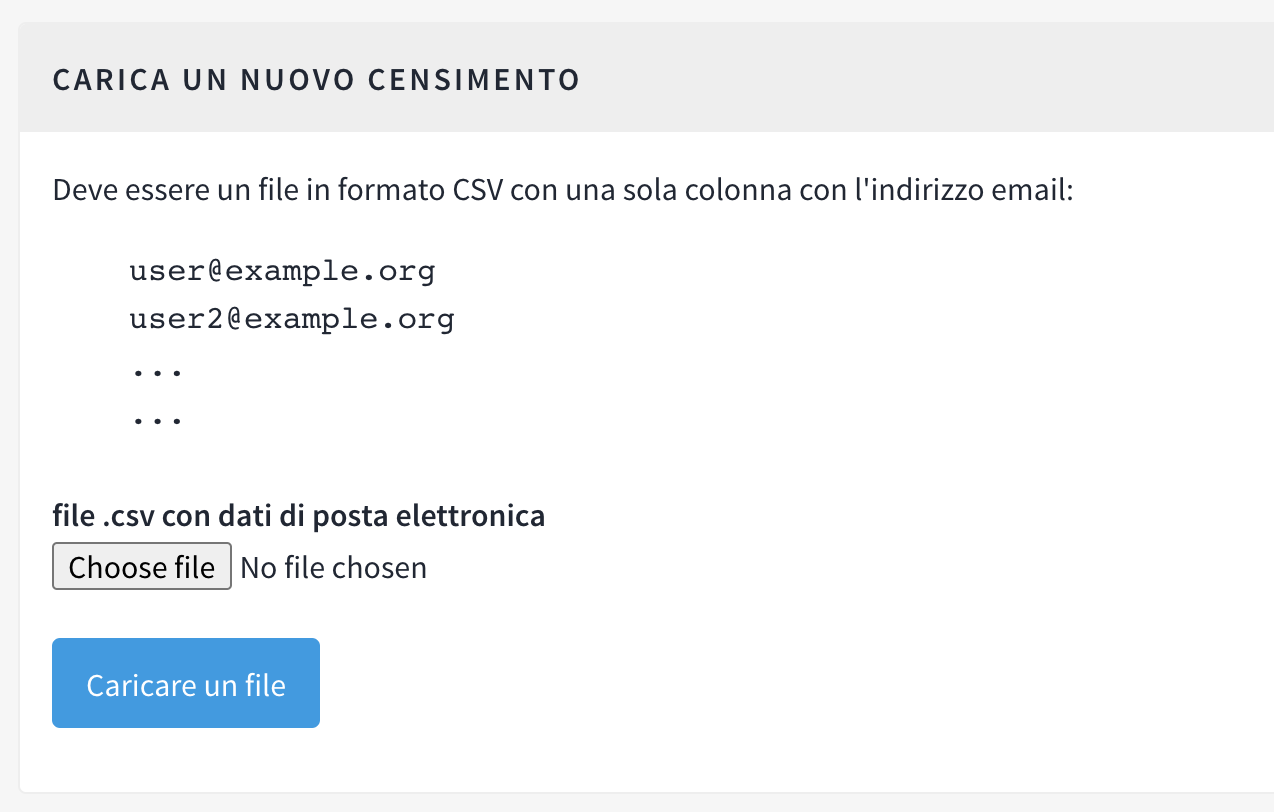
\includegraphics[width=0.50\textwidth]{auth}
  \end{wrapfigure}

  Per gestire l'autenticazione si potrebbe importare all'interno di Decidim una lista di mail possedute dall'azienda.

  (ad esempio quelle registrate all'interno degli "sportelli" online dell'azienda e quindi validate)

\end{frame}

\begin{frame}{Problematiche minori - Upload di immagini}
  \begin{wrapfigure}{r}{0.50\textwidth}
    \centering
    
\includegraphics[width=0.50\textwidth]{immagine}
  \end{wrapfigure}
  Sarebbe comodo un tool per il ridimensionamento delle immagini


  o quantomeno sapere quali siano i limiti di dimensione delle immagini


\end{frame}



{\setbeamercolor{palette primary}{fg=white, bg=mLightBrown}
\begin{frame}[standout]
  Demo!

\end{frame}
}
